% !TeX spellcheck = en_GB
\section{Evaluation}
\subsection{Size of the Diamond}

One we have find our calibration factor for our microscope defining the size of  diamond just require the pixel number in it. For counting the pixel FIJI software was used in two different ways (see figure \ref{fig:diasize4}). The first was overlay a circle that matched the area of the bright diamond and the second was measure the diameter of it with a cross section line. In both cases the size in pixels was really similar, $D=34\pm1 pixel$ as shown in the next figure. Multiplied by our preview calibration factor lead to $D_{diamond}=24\pm4 \mu m$
\begin{figure}
	\centering
	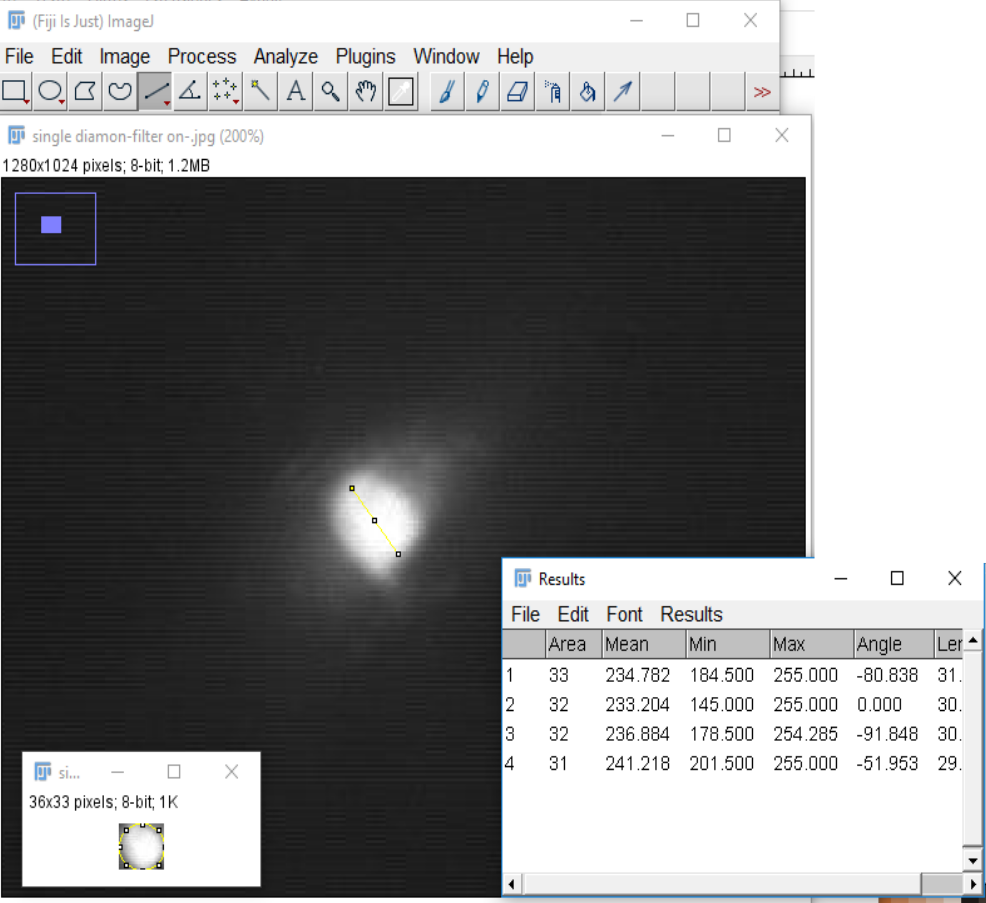
\includegraphics[width=0.7\linewidth]{../figures/Diasize4}
	\caption[sizediam]{Picture of the Software use to the pixel measurement, in the bottom left the measurement with the overlay of circles and in the right the measurement with a direct line.}
	\label{fig:diasize4}
\end{figure}


\subsection{Fluorescence Spectrum}
As indicated in section \ref{sec:nvcentres} the NV-centres exist in a NV$^-$ and a NV$^0$ state. While the ODMR-measurements can only be done on the NV$^-$ state we need to make sure that the diamond we found has NV$^-$ centres inside.\\

Therefore the fluorescence spectrum of the diamond is recorded and the position of the ZPL is determined. In figure \ref{fig:fluorescence} we see the ZPL to be at the position $\lambda_\text{ZPL}=(645\pm3)\,\mathrm{nm}$ which corresponds to an energy of $E_\text{ZPL}=(1.922\pm0.009)\,\mathrm{eV}$. This corresponds roughly to the energy given in figure \ref{fig:nvcentres}. So we verified the existence of NV$^-$ centres in the found diamond.
\begin{figure}
	\centering
	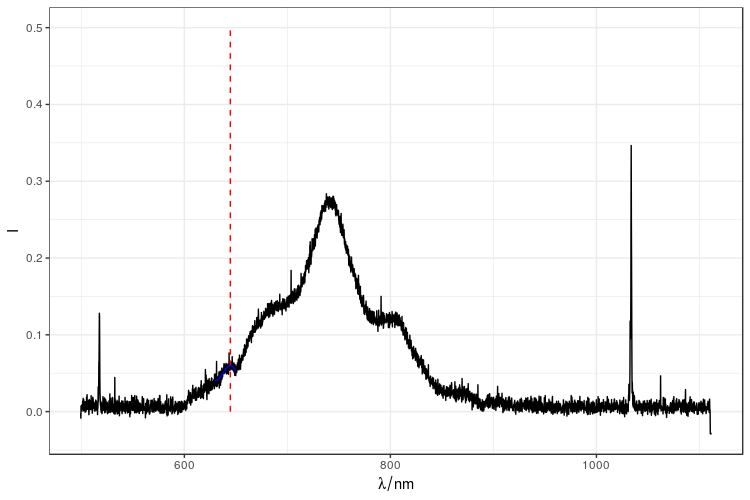
\includegraphics[width=0.8\textwidth]{../figures/fluorescence.png}
	\caption[Fluorescence spectrum of the diamond]{Fluorescence spectrum of the diamond with the zero phonon line (red line) at $\lambda_\text{ZPL}=(645\pm3)\,\mathrm{nm}$. The spectrum was achieved by averaging over 10 measurements.}
	\label{fig:fluorescence}
\end{figure}

\subsection{ODMR Measurements}

The ODMR Measurements were conducted without a magnetic field and afterwards with three magnetic fields pointing into different directions. The measured ODMR spectrum without a magnetic field is shown in figure \ref{fig:odmr-no-B}. The resonance frequency in this spectrum is determined to be $f_\text{resonance}=(2.8699\pm0.0002)\,\mathrm{GHz}$ using the calibration done in section \ref{sec:odmr-cal}.\\

In figure \ref{fig:odmr-magnet} the ODMR measurements with enabled magnetic fields are displayed. In figure \ref{fig:odmr-magnet-x} and \ref{fig:odmr-magnet-y} one can see one, respectively two resonance pairs while in \ref{fig:odmr-magnet-z} we can barely identify some peaks but cannot assign them to resonance pairs so we discarded this measurement.\\

The peaks in figure \ref{fig:odmr-magnet-x} and \ref{fig:odmr-magnet-y} we can assign to resonance pairs but the centre frequency of this resonance pairs is not equal to the measured resonance frequency of the $B=0$-measurement shown in figure \ref{fig:odmr-no-B}. So to calculate the resonance frequencies and with this the magnetic fields we used the measured frequency. Possible reasons for the shifting of this energy are explained in section \ref{sec:summary}.

\begin{figure}
	\centering
	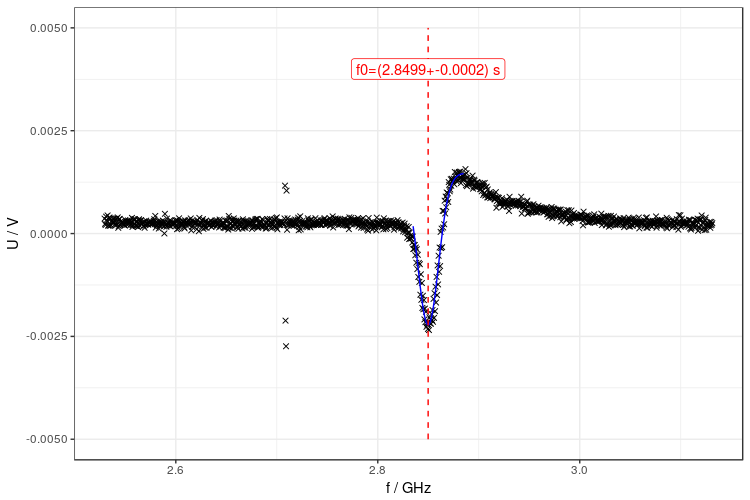
\includegraphics[width=0.8\textwidth]{../figures/odmr-1.png}
	\caption{ODMR Measurement of the diamond without a magnetic Field}
	\label{fig:odmr-no-B}
\end{figure}


\begin{figure}
	%\centering
	\begin{subfigure}{0.5\textwidth}
		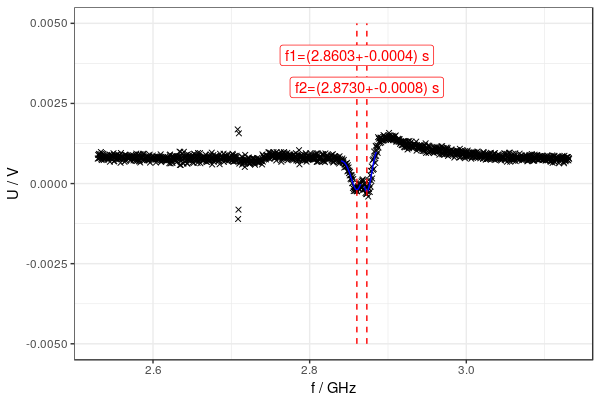
\includegraphics[width=\textwidth]{../figures/odmr-bx.png}
		\subcaption{Magnetic field in $x$-Direction}
		\label{fig:odmr-magnet-x}
	\end{subfigure}
	\begin{subfigure}{0.5\textwidth}
		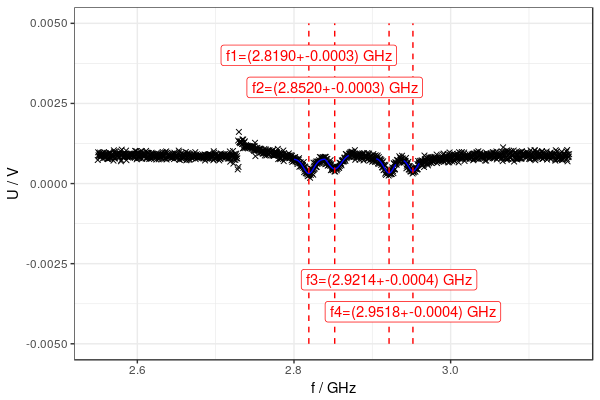
\includegraphics[width=\textwidth]{../figures/odmr-by.png}
		\subcaption{Magnetic field in $y$-Direction}
		\label{fig:odmr-magnet-y}
	\end{subfigure}
	\begin{subfigure}{0.5\textwidth}
		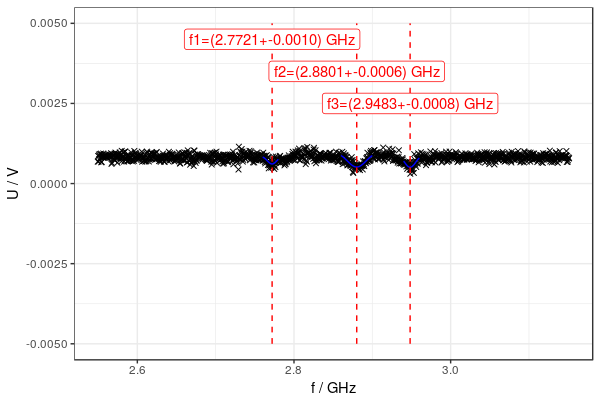
\includegraphics[width=\textwidth]{../figures/odmr-bz.png}
		\subcaption{Magnetic field in $z$-Direction}
		\label{fig:odmr-magnet-z}
	\end{subfigure}
	\caption{ODMR spectrum within a magnetic field}
	\label{fig:odmr-magnet}
\end{figure}

\begin{table}
	\centering
	\begin{tabular}{c|c|c}
		&Resonance 1&Resonance 2\\\hline
		$f_x / \mathrm{MHz}$&$6.2\pm0.5$&-\\
		$f_y / \mathrm{MHz}$&$34.7\pm0.4$&$66.5\pm0.4$\\\hline
		$B_x / \mathrm{mT}$&$0.214\pm0.018$&-\\
		$B_y / \mathrm{mT}$&$1.197\pm0.014$&$2.297\pm0.014$\\\hline
		$d_x/d$&$0.036\pm0.003$&-\\
		$d_y/d$&$0.203\pm0.002$&$0.389\pm0.002$
	\end{tabular}
	\caption{Resonance Pairs}
\end{table}